\documentclass{standalone}
\usepackage{graphicx}
\usepackage{caption}
\usepackage{float}
\usepackage{varwidth}
\usepackage[export]{adjustbox}

\begin{document}

\centering
\begin{minipage}[t]{0.45\textwidth}
    \textbf{A}\\[4pt]
    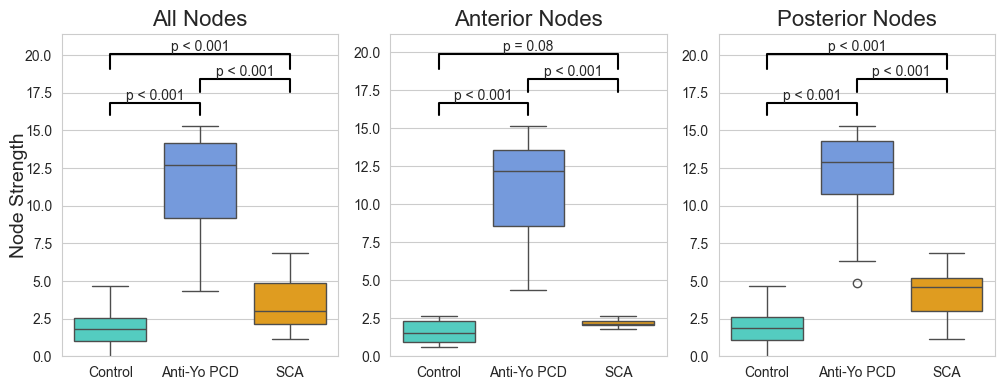
\includegraphics[width=\textwidth]{graphics/node_strength.png}
\end{minipage}
\begin{minipage}[t]{0.45\textwidth}
    \textbf{B}\\[4pt]
    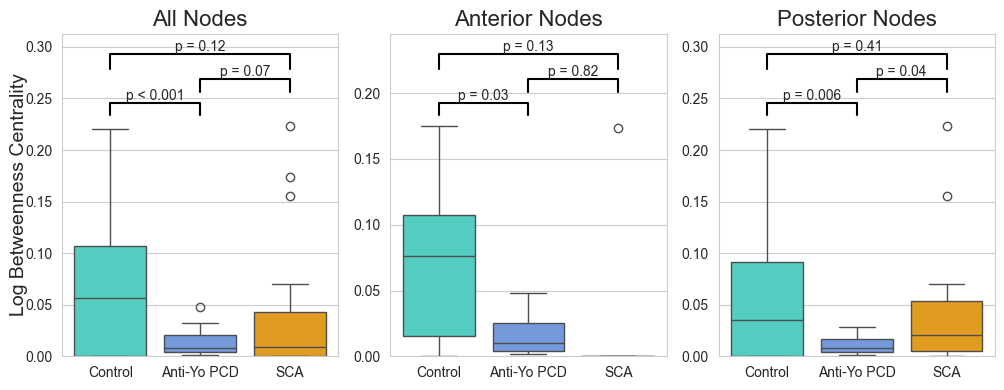
\includegraphics[width=\textwidth]{graphics/betweenness.png}
\end{minipage}
\begin{minipage}[t]{0.45\textwidth}
    \textbf{C}\\[4pt]
    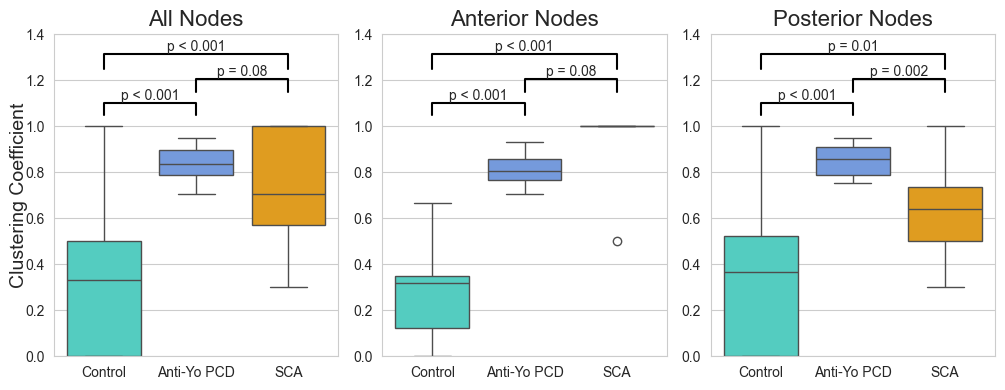
\includegraphics[width=\textwidth]{graphics/clustering_coefficient.png}
\end{minipage}
\begin{minipage}[t]{0.45\textwidth}
    \textbf{D}\\[4pt]
    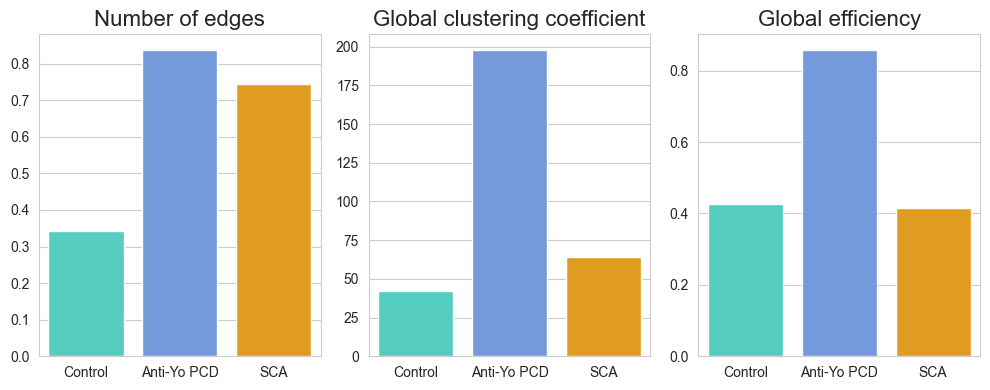
\includegraphics[width=\textwidth]{graphics/barplots_graph.png}
\end{minipage}

\end{document}